\documentclass{deliverablereport}
\usepackage[final]{pdfpages}

\deliverable{component-architecture}{smc-documentation}
\deliverydate{02/28/2017}
\duedate{02/28/2017 (Month 18)}
\author{Erik Bray}
\renewcommand{\SMC}{\software{SMC}}

\begin{document}
\maketitle
\strut\githubissuedescription
\newpage\tableofcontents\newpage

\section{Introduction}

\software{SageMathCloud} (\SMC) was presented as an emerging technology in
\delivref{dissem}{techno}. It is an on-line open source platform which allows
the creation of collaborative scientific projects. Each user can create
\emph{projects} within the platform. Each project is hosted on a \Linux virtual
machine accessed through a web interface and provides access to many scientific
tools.  It is thus an important working example of a Virtual Research
Environment (VRE) as described in Section 1.3.2 of the Proposal, with
capabilities suitable for reasearchers, software developers, and teachers.
Launched in 2013, \SMC presently hosts over 400,000 projects and nearly 20,000
weekly active users. This fast adoption by a wide variety of users demonstrates
the relevance and the long term impact this kind of collaborative environment
can have.  Although it is just one example of a VRE, it serves as an important
prototype for OpenDreamKit (ODK).

Because there is no one VRE that suits all needs, a framework for VREs must be
highly flexible, allowing researchers to choose from the tools that best suit
the task and combine them in arbitrary, yet interoperable ways.  \SMC has
already taken steps in this direction by providing a unified interface to
software systems such as \Sage, \GAP, and other ODK components, as well as a
full \Linux shell with common software development tools, \LATEX document
editing and display, \Jupyter notebooks, computing resources, and other
capabilities that one would need for a VRE with unlimited possibilities.  While
there is still work to be done on further integrating the components of \SMC,
this is work that ODK can feed back into \SMC while simultaneously using \SMC
as an example VRE.

Another major effort in building a VRE, beyond innovations on the environment
itself and development of effective workflows within a VRE, is the underlying
software and computing infrastructure needed to make VREs accessible and widely
available.  \SMC has given us a real working example, with open source code, of
how to build a cloud-based VRE, accessible from a web browser from anywhere in
the world, with a consistent user interface around its components.  There are
many technical details we can learn from it, such as what software technologies
its framework is built on, and how its underlying computing resources are
organized and administered.

The purpose of this deliverable is to better understand the technical details
of how \SMC works, so that the ODK members can learn from it, and also
eventually contribute innovations from ODK project back into \SMC.

\section{History of \SMC's development}

%% Provide a brief history of \SMC's development, and why it is difficult to
%% document, and difficult for newcomers to contribute to.
William Stein, the creator of \Sage and \SMC, started working on \SMC in 2012
as a way to make \Sage -- notoriously non-trivial to install -- more accessible
to users via a cloud service.  Around the same time, it became apparent that,
in order to survive and to compete with commercial mathematical software
systems, it would be extremely helpful to have a self-sustained income stream
based around \Sage.  Stein realized that, with enough value-added on top of
\Sage itself, users might be willing to pay for access (and in particular
computing and network resources) for this service.  So \SMC became more than
just \Sage, but rather a cloud-based research and teaching environment built in
large part around but not solely focused on \Sage.

For most of its development history, Stein has been \SMC's sole developer,
working in his spare time while being a professor at the University of
Washington at Seattle.  It was not until September 2013 when its second most
extensive contributor, Harald Schilly, made his first commit to the \SMC source
code repository.  Since then, especially once the code was made open source in
Fall 2015, a little more than two dozen people have made developments.
Nevertheless Stein still has done more than ten times as much work (roughly, in
terms of number of repository commits) than anyone else on the project, and as
such is the only person who truly understands its full design.

Because it has had effectively one developer, and because of the breakneck pace
at which it was built, very little of \SMC's internal design--both overall and
the lower-level details-- is documented in an accessible manner.  In order to
understand \SMC's design, one currently has to read the code, and get inside
Stein's head a little bit to understand how he might have been thinking.
Further complicating matters is that \SMC has gone through multiple partial
rewrites (most notably a rewrite of the server code, originally in \Python, to
\JavaScript).  Because these rewrites have been only partial (due to Stein's
limited time and developer resources), this has resulted in what amounts to
layers of digital sediment that must be sifted through carefully in order to
understand how and why some design decisions came about.

Because of the fast pace of development, documentation on how to help with
development of \SMC itself--something of interest if ODK is to contribute back
to \SMC--has also fallen behind.  Even the talk
\href{https://youtu.be/GOuy07Kift4}{How to contribute to SageMathCloud} given
by William Stein in late 2015 and mentioned in the report for
\delivref{dissem}{workshops-1} is no longer \emph{as} useful for getting
started on full stack development of \SMC as it was a year before this report
(though it still contains some helpful information).

None of this should be read as criticism of Stein or \SMC--the reasons for the
relative opacity of \SMC's design are understandable.  It is just helpful to
understand why it is particularly challenging to understand and document this
already enormously complex piece of software.  An additional challenge of this
task is to write documentation and development procedures that will be
maintainable through future development without always becoming immediately
obsolete.

\begin{figure}
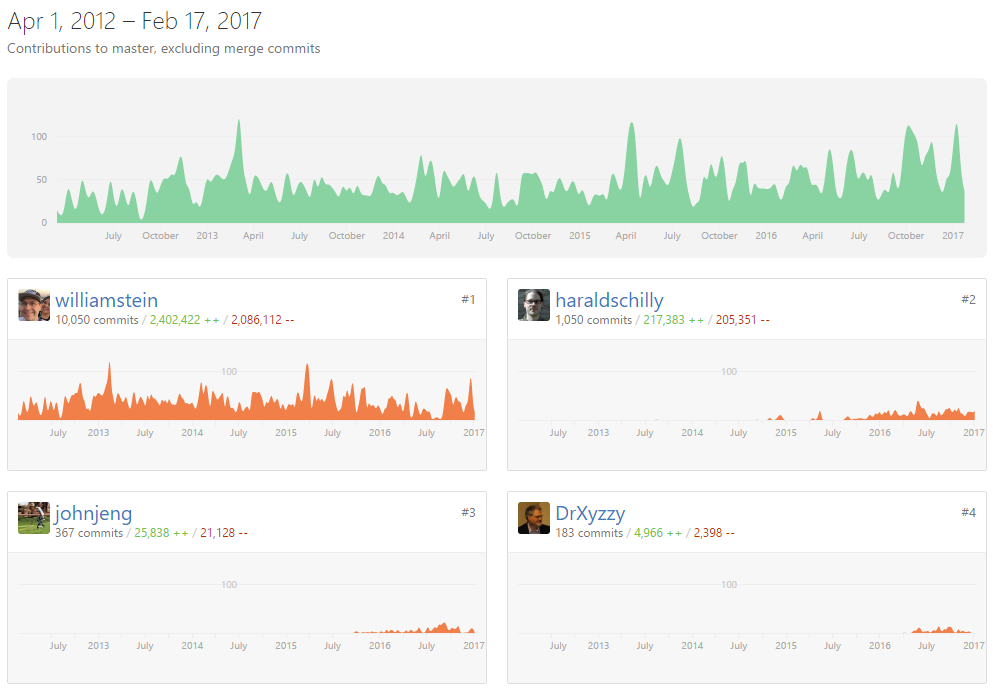
\includegraphics[width=\textwidth]{images/smc-contributions-2017-02-17.png}
\caption{top \SMC source contributors from the project's beginning in 2012 through February 2017}
\end{figure}

\section{Current state of \SMC's source code and documentation}

%% Summarize the current state of the source code, the current state of the
%% architecture documentation, and of the development documentation and
%% resources.  This is really "where the work started from".
\SMC's source code currently resides in a single \software{git} repository
hosted on GitHub.  This repository contains all code written uniquely for
\SMC--web-based frontend and all backend servers--as well as scripts and tools
for development of \SMC.

It also has a collection of many small scripts and utilities used for managing
the live \SMC site and the many servers that comprise it (hubs, compute nodes,
etc.)  Many of these are just single command-line commands for what might be
common tasks.  However, there is little to no documentation for most of these
tools or when and how they should be used.  Most of them are not directly
relevant to doing development of \SMC.

Most of the main \SMC source code is split across two \Python packages, five
\JavaScript packages, and one directory containing additional web resources
such as fonts and images, as well as "vendored" \JavaScript--third-party source
code that may require special handling to integrate into the \SMC web app.

There is also a configuration script for
\href{https://webpack.github.io/}{Webpack}, a tool used to bundle \JavaScript
sources, HTML, images, and other resources into a working website.  This file
serves as something of a map to how all of \SMC's frontend code fits together.
Because there is no equivalent for the backend, it is a little more difficult
at first to understand how the server-side code works.  That said, the general
layout is clear enough that an experienced developer, equipped with high-level
documentation of \SMC's infrastructure, can gain insight into what features
might be implemented where.  More such high-level documentation is needed,
however.

Beyond a few brief "README" files in the main source packages, and scattered
in-line documentation in some of the source files, there is very little
documentation of what each source file is or what internal or external APIs
might exist.  So while the high-level structure is not difficult to understand,
it is somewhat more difficult to understand the flow of data and program
control.

\section{Documenting \SMC's internal design}

%% Provide a brief summary of my documentation of \SMC's internals, with link
%% to the full documentation.  Explain how this should help others understand
%% how \SMC works, even given its relative flux.  Discuss future work needed
%% to understand the source code and its modularization.
In order to help newcomers better undertand \SMC's internal design, we have
begun documenting some aspects of it in better detail.  The first version of
this document is included as Appendix \ref{app:doc} of this report. It has also
been accepted into
\href{https://github.com/sagemathinc/smc/blob/master/src/doc/design_overview/overview.rst}{SMC's
source code repository} for easier discovery by anyone interested in how \SMC
works.

This document covers two topics in particular: It goes into greater detail than
any previous documentation on the core \JavaScript libraries and tools that
\SMC is built on, including a brief introduction to those tools, and some
discussion of how and why they are used by \SMC.  This list is still not
exhaustive, but it covers most of the key technologies one needs to have
understanding of in order to understand \SMC's code base.

Our documentation also provides a brief tour through \SMC's code base--
specifically the client-side code--explaining step by step how a page is
rendered by \SMC's client-side code.  This explains specific examples from
\SMC's code base of how its dependencies are used, and how the source code is
organized internally.  Some of the exact details may change in the future, but
the basic design (at least on the client side) is likely to remain stable for
some time.  This is due in part to the mostly finished work of rewriting \SMC's
web client on top of React--a \JavaScript UI framework created and heavily
supported by Facebook.  This React-based design is not likely to change in the
forseeable future.

The walkthrough we have written on \SMC's code base is for a very simple
example.  For future work, it would be instructive to include a more complex
example, such as a walkthrough of how \SMC's advanced real-time documentation
collaboration features work.  A detailed walkthrough of the server-side
code-base is still needed as well, but Stein and Schilly are in the process of
significantly reorganizing much of that code. Thus it would be advisable to
wait until more of that work is complete before writing further detailed
documentation.


\section{Overview of \SMC's software development process}
%% Summarize work done improving development processes and explain ongoing
%% and future work needed in this area.
A large, complex web application like \SMC is non-trival to do development on
compared to more self-contained software projects.  A full \SMC deployment
consists of multiple server processes that must work in concert, and other
moving parts such as Webpack builds for assembling the web client.  \SMC's
source code documents a few different ways to work on \SMC:

\begin{itemize}
    \item The simplest is to run a development \SMC server directly on one's
        personal computer, reloading the server as necessary while making
        changes to the source code.  \SMC in fact has a "development" mode
        wherein all of \SMC's server components run on one's local machine,
        which also acts as the sole compute node.  Any projects on the
        development server are created and run on the local machine, under the
        developer's login account.  This is certainly the simplest way to work,
        but the code currently has some (known) bugs such that a \SMC server
        run in this way is not actually fully functioning.  Thus, while this is
        feasible for some development tasks, it is not currently possible to
        develop the full \SMC stack in this way.  We recommend trying to fix
        that if at all possible.  Another downside to this method is that the
        developer must install all of \SMC's requirements manually, and this is
        not well documented at the moment.  As much of \SMC is UNIX-oriented
        this also creates a barrier for would-be developers working on Windows.

    \item Another compelling way to develop on \SMC is referred to as
        "SMC-in-SMC".  It is possible, on an existing \SMC server (particularly
        the main one hosted at {\tt cloud.sagemath.com}) to download the \SMC
        source code into a project hosted on that server and run a full \SMC
        server from within the project.  This is somewhat similar to the
        previous method, but takes advantage of the fact that all of \SMC's
        runtime dependencies are already available inside an \SMC project.  It
        is easier to get \SMC-in-SMC up and running than most other methods,
        and it works impressively well considering its recursive nature.  While
        one is restricted to working within an \SMC project this is not
        \emph{much} of a downside considering the flexibility afforded to \SMC
        users).  It does, however, require having a non-free \SMC account (the
        default free accounts for \SMC do not allow internet access from within
        projects), though Stein is generous in giving less restricted free
        accounts to users who wish to help with \SMC development.

    \item The easiest way to get a fully functioning \SMC server up and running
        on one's personal computer is with the official Docker container for
        \SMC (see the report for
        \delivref{component-architecture}{virtual-machines} for more
        information on Docker containers).  The Docker container image is
        well-maintained to work with the latest \SMC source code, and provides
        a turn-key solution for a full-stack single-server \SMC deployment.
        There is a slight downside, however, that its current design is not
        very amenable to development.  For example, the \SMC source code is
        contained in the container itself, which means any and all development,
        including editing the source code, must be done within the Docker
        container.  This may require a would-be developer to manually reproduce
        their preferred software development environment (tools and settings)
        and edit all source code directly inside the Docker container.  A
        better approach is to design a Docker container for development that
        allows the developer to keep the \SMC source code on their local
        machine.  The \SMC Docker container would then mount the source code as
        an external "volume" (this is a feature of containers similar to a
        shared folder between the container and its host).  The developer can
        than do all development work on their local machine, but \emph{execute}
        the source code inside the Docker container, freeing them of the need
        to worry about setting up \SMC's dependencies.  We have begun work on a
        development-friendly Docker container for \SMC, but more work is
        required to make this fully viable.  When completed, this will likely
        be the easiest way for anyone to get quickly up and running with \SMC
        development on their personal computer.

\end{itemize}


\section{Conclusion and future work}
%% Conclude with summary of where we started, where we are now, and what work
%% is still needed.  Perhaps raise open questions about whether or not D3.4, as
%% currently documented in the proposal, is worth pursuing, and why/why not.
Prior to work on this deliverable there was scant documentation on \SMC, its
overall design, its dependencies, or its internals.  There was some
documentation on how to do development on it, but not enough, and sometimes out
of date.  With the documentation we have added it should require less effort
for a motivated developer to gain the necessary background knowledge (such as
knowledge of the core technologies \SMC is built on) to do development on \SMC.
Our documentation should also help lead to a faster understanding of the
general flow of \SMC's design, though it would not have been feasible to
document the implementations of all of its features.  Some of its more advanced
features--especially key features such as its real-time collaborative document
editing--do require further documentation.  More documentation is needed on the
design of \SMC's server components, though that work should wait until their
implementation details have stabilized more.

We have also gained experience within the ODK team on setting up a \SMC server
and the process of doing development on \SMC.  Gaining this shared knowledge is
a prerequisite for future work on determining what aspects of \SMC--at its core
a framework for cloud-based hosting of complex mathematical software, and thus
a powerful tool for building VREs--can be integrated into ODK.  However,
further work is needed on improving the development tools for \SMC--in
particular we recommend improving the existing Docker container for \SMC for
development on one's personal computer.


\appendix
\section{\SMC documentation overview}
\label{app:doc}

Please find attached the document that was produced as part as the deliverable
objective.  It is also available on-line at this address:
\url{https://github.com/sagemathinc/smc/blob/master/src/doc/design_overview/overview.rst},
that is, inside the source code repository of \SMC.

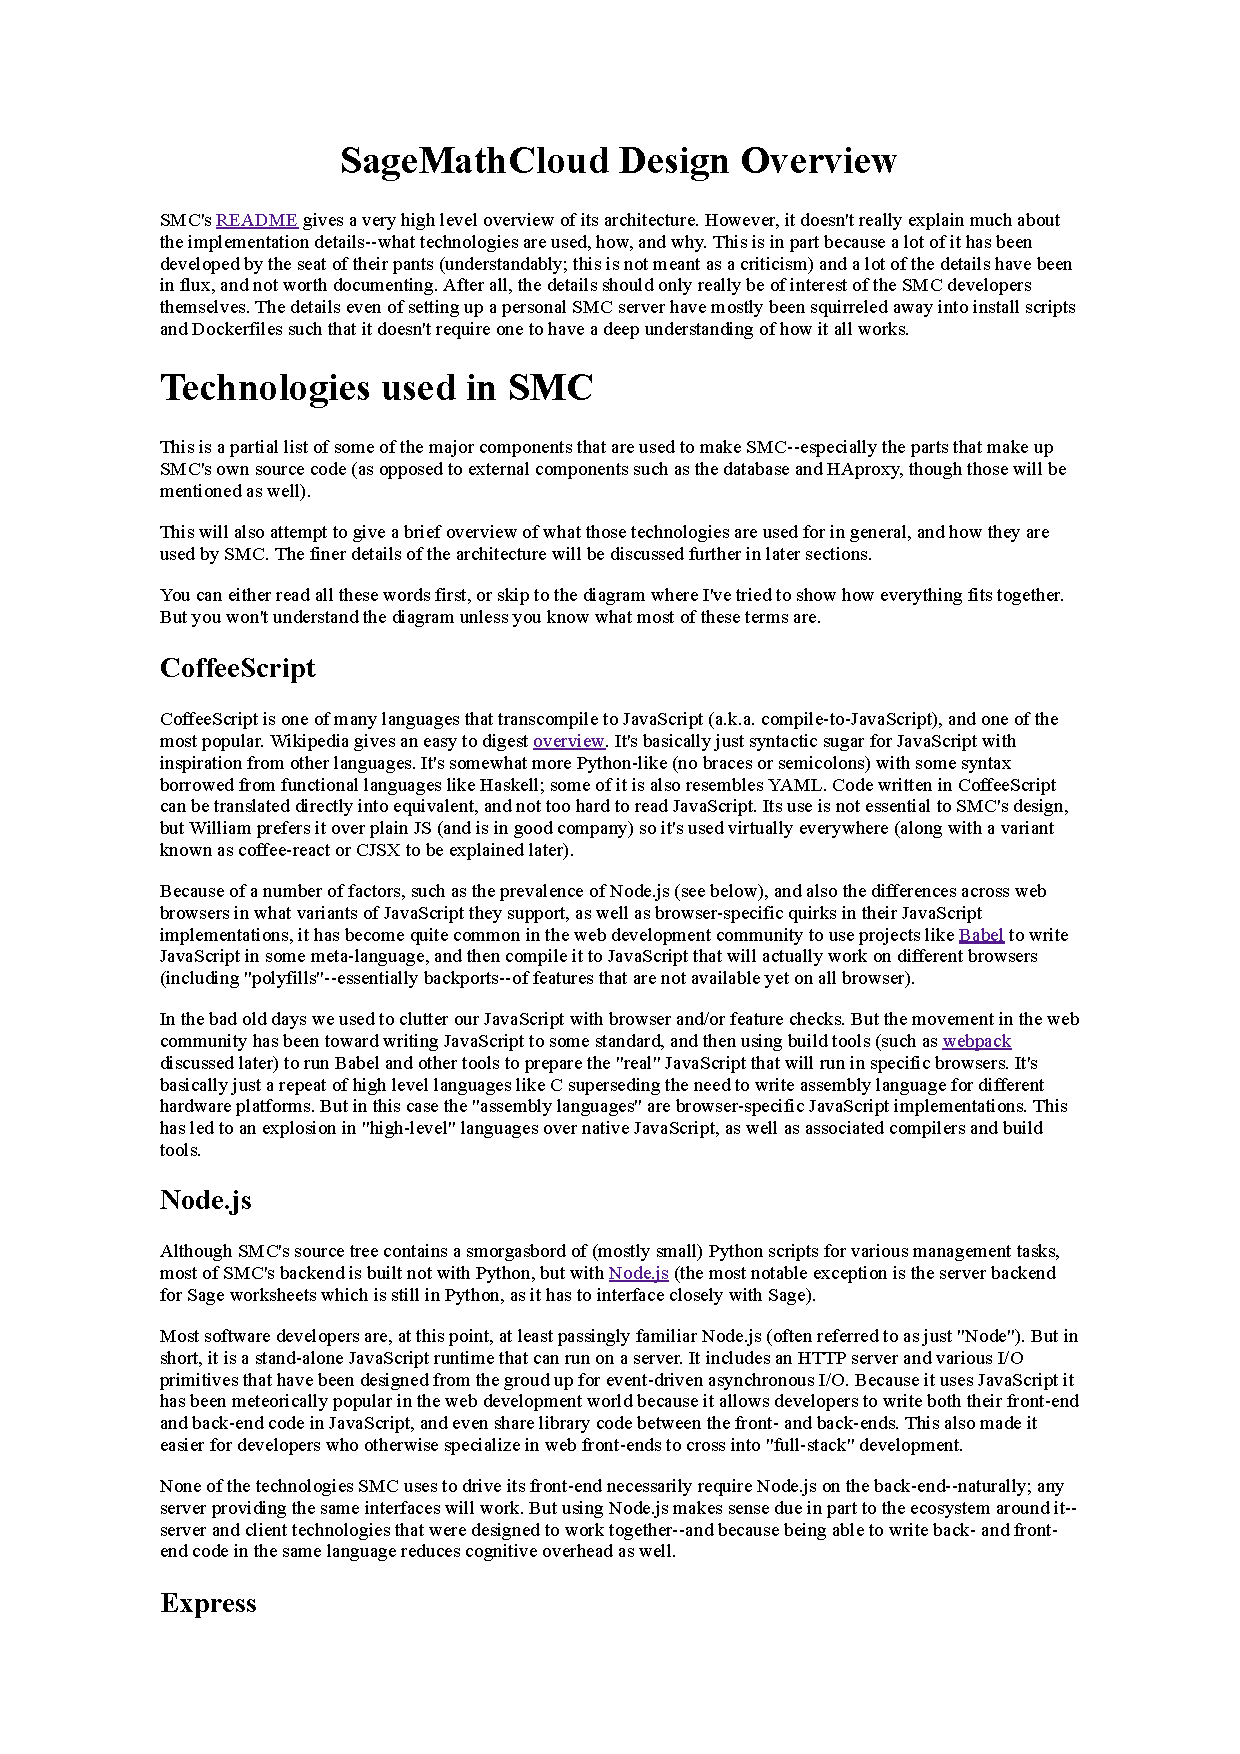
\includepdf[pages=-]{overview/overview.pdf}
\end{document}

%%% Local Variables:
%%% mode: latex
%%% TeX-master: t
%%% End:

%  LocalWords:  githubissuedescription newpage tableofcontents newpage printbibliography
